\documentclass[11pt, a4paper,twocolumn]{jarticle}
\usepackage[dvipdfmx]{graphicx}

\begin{document}
%=============================================================
\section{Understanding AD,DA conversion , and C programing for controlling AD/DA conversion ($2^{nd} day$)}
\subsection{Purpose}
今回の実験ではアナログからデジタル,デジタルからアナログへの信号変換をコンピューターを用いて行うことが目的である.
\subsection{Procedure}
\noindent
\textbf{Task 2.1 DC信号の取り込み}

乾電池により作り出した直流電源のDC信号をAD/DAボードでパソコンに取り込み(AD変換),取り込んだファイルをテキストファイルとして出力する.
テキストファイルをエクセルにより描画して電圧の推移を調べる.
その変化量より量子化について考える.

\noindent
\textbf{Task 2.2 時間変化する信号の取り込み(サンプリング定理)}

ファンクションジェネレーターによって正弦波を出力し,その電圧を10Hz,50Hz,100Hzのサンプリング周波数で取り込む.
また取り込んだ値をエクセルにより描画する.
この操作をファンクションジェネレーターで10Hz,20Hz,50Hzの三種類の正弦波について行う.
この際波形の確認はオシロスコープを用いて確認を行う.

\noindent
\textbf{Task 2.3 DA変換}

Cプログラムにより"ド"と高い"ド"の音階の周波数それぞれ262Hz,523Hzを発生させそれをオシロスコープにより観測した.

\subsection{Result}
%==============================================
\noindent
\textbf{Task 2.1}

実験の結果以下のようなグラフが得られた.

\begin{figure}[htbp]
 \begin{center}
  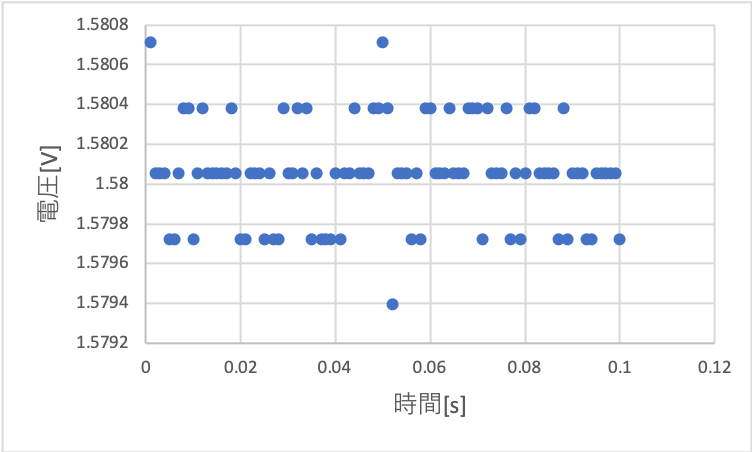
\includegraphics[width=0.8\linewidth]{fig2.png}
 \end{center}
 \caption{乾電池のAD変換}
 \label{fig:2}
\end{figure}

また最小値を0に設定した際は以下のようになる.

\begin{figure}[htbp]
 \begin{center}
  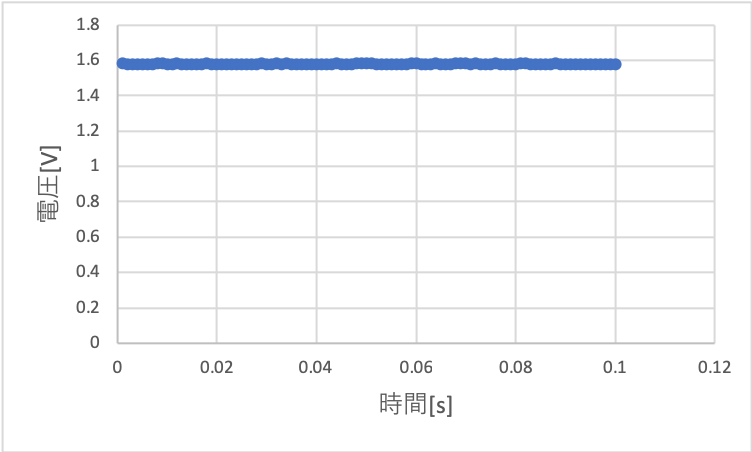
\includegraphics[width=0.8\linewidth]{fig3.png}
 \end{center}
 \caption{乾電池のAD変換(2)}
 \label{fig:3}
\end{figure}

この結果より乾電池の電圧は一定値を取ることが読み取れる.
%==============================================

\noindent
\textbf{Task 2.2} \\
測定の結果それぞれの正弦波について以下のようなグラフが得られた.

\begin{figure}[htbp]
 \begin{center}
  \includegraphics[width=0.8\linewidth]{fig4.png}
 \end{center}
 \caption{sin波(10Hz),サンプリング周波数(10Hz)}
 \label{fig:4}
\end{figure}

\begin{figure}[htbp]
 \begin{center}
  \includegraphics[width=0.8\linewidth]{fig5.png}
 \end{center}
 \caption{sin波(10Hz),サンプリング周波数(50Hz)}
 \label{fig:5}
\end{figure}

\begin{figure}[htbp]
 \begin{center}
  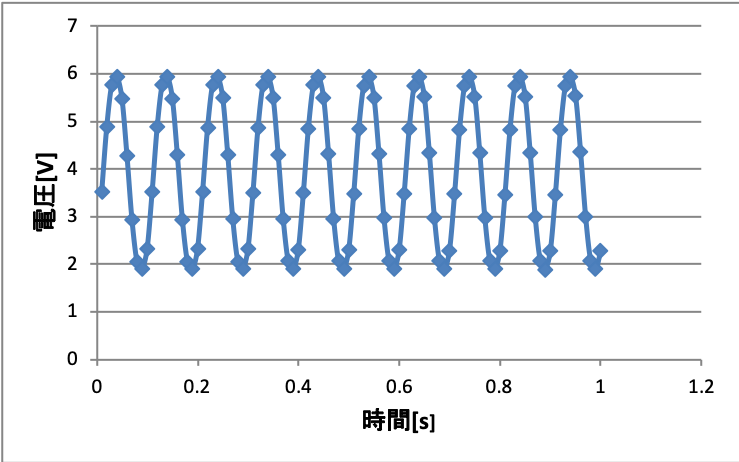
\includegraphics[width=0.8\linewidth]{fig6.png}
 \end{center}
 \caption{sin波(10Hz),サンプリング周波数(100Hz)}
 \label{fig:6}
\end{figure}

\begin{figure}[htbp]
 \begin{center}
  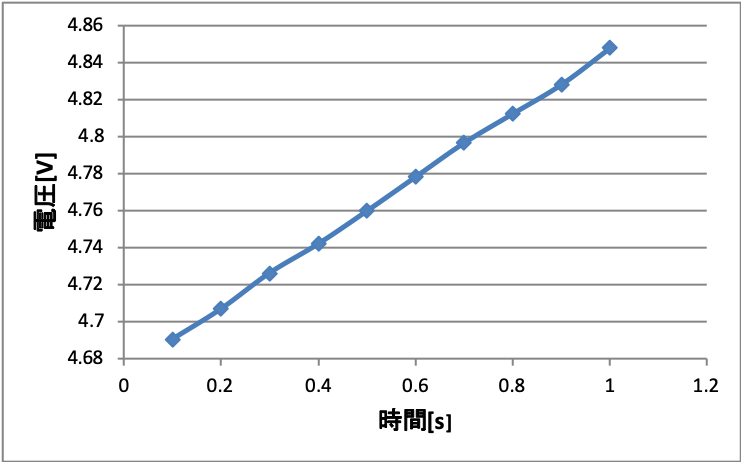
\includegraphics[width=0.8\linewidth]{fig7.png}
 \end{center}
 \caption{sin波(20Hz),サンプリング周波数(10Hz)}
 \label{fig:7}
\end{figure}

\begin{figure}[htbp]
 \begin{center}
  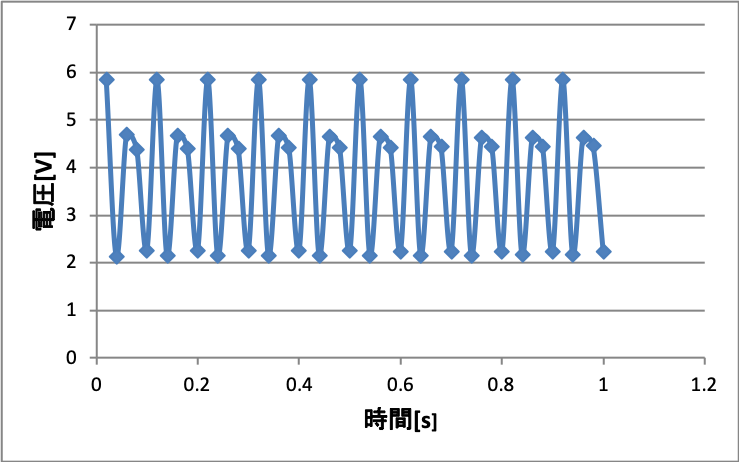
\includegraphics[width=0.8\linewidth]{fig8.png}
 \end{center}
 \caption{sin波(20Hz),サンプリング周波数(50Hz)}
 \label{fig:8}
\end{figure}

\begin{figure}[htbp]
 \begin{center}
  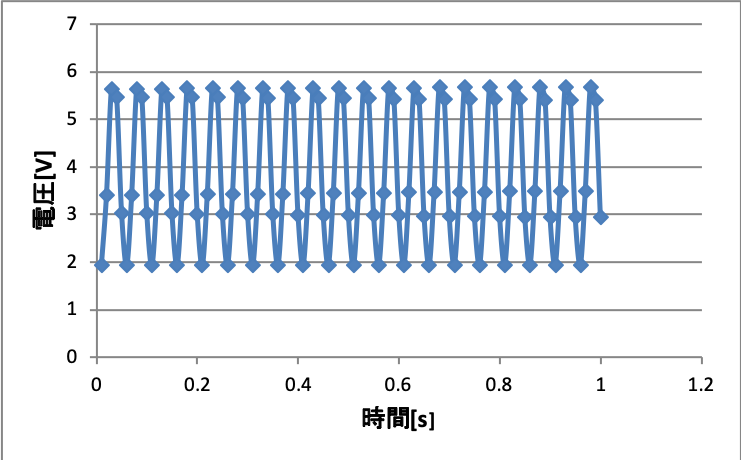
\includegraphics[width=0.8\linewidth]{fig9.png}
 \end{center}
 \caption{sin波(20Hz),サンプリング周波数(100Hz)}
 \label{fig:9}
\end{figure}

\begin{figure}[htbp]
 \begin{center}
  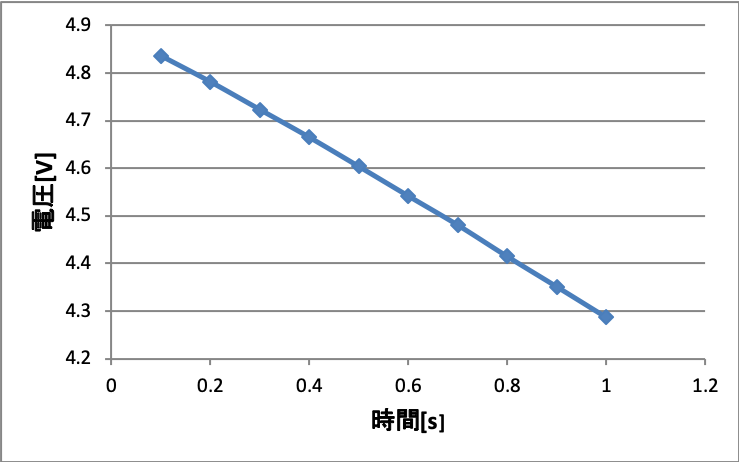
\includegraphics[width=0.8\linewidth]{fig10.png}
 \end{center}
 \caption{sin波(50Hz),サンプリング周波数(10Hz)}
 \label{fig:10}
\end{figure}

\begin{figure}[htbp]
 \begin{center}
  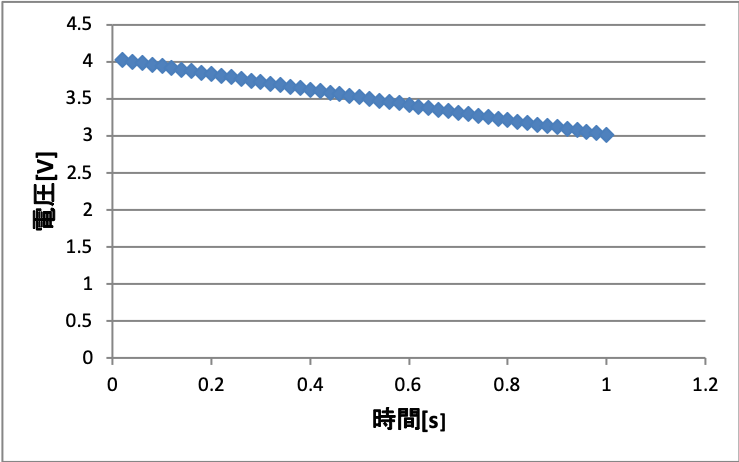
\includegraphics[width=0.8\linewidth]{fig11.png}
 \end{center}
 \caption{sin波(50Hz),サンプリング周波数(50Hz)}
 \label{fig:11}
\end{figure}

\begin{figure}[htbp]
 \begin{center}
  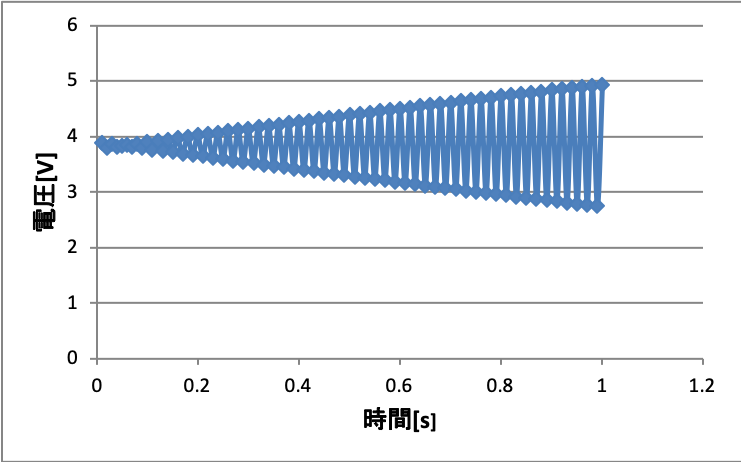
\includegraphics[width=0.8\linewidth]{fig12.png}
 \end{center}
 \caption{sin波(50Hz),サンプリング周波数(100Hz)}
 \label{fig:12}
\end{figure}

\newpage

\noindent
\textbf{Task 2.3 DA変換}
実験よりオシロスコープから得られた波形を以下に示す.
\begin{figure}[htbp]
 \begin{center}
  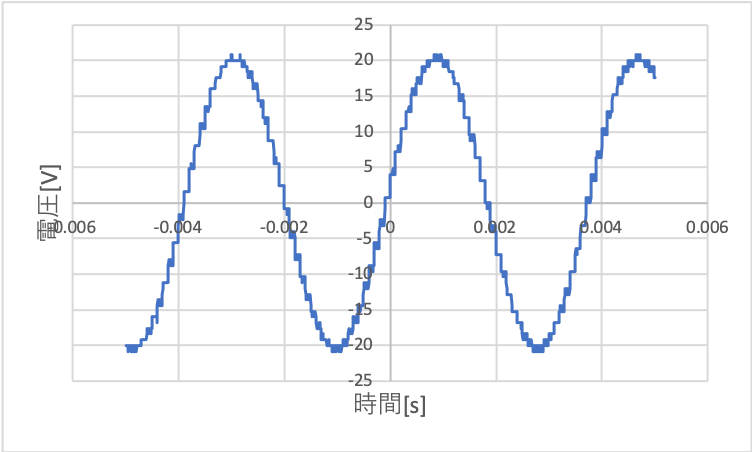
\includegraphics[width=0.8\linewidth]{fig13.png}
 \end{center}
 \caption{sin波(262Hz),サンプリング周波数(10kHz)}
 \label{fig:13}
\end{figure}

\begin{figure}[htbp]
 \begin{center}
  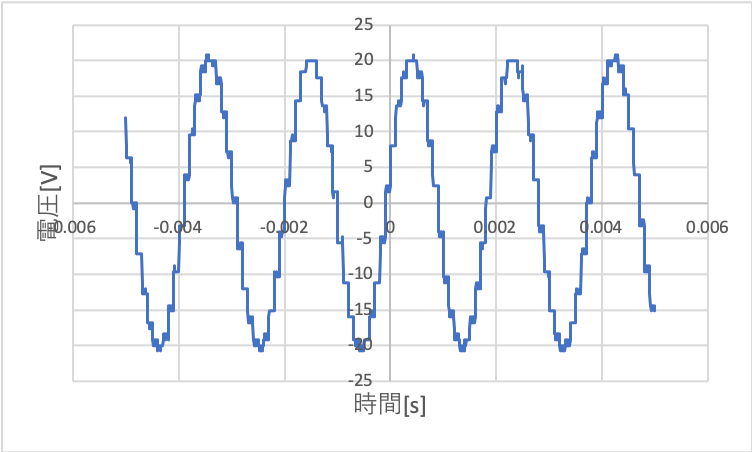
\includegraphics[width=0.8\linewidth]{fig14.png}
 \end{center}
 \caption{sin波(523Hz),サンプリング周波数(10kHz)}
 \label{fig:14}
\end{figure}

\subsection{Discussion}
\noindent
\textbf{Task 2.2} \\
電池の電圧は1.5Vで一定値を取るため正しく測定できたことが予想できる.
またグラフは0.0003Vごとに離散値を取ることが読み取れる.
これは今回使用したNational Instrumentsの計測器が16bitの制度を持ち今回のプログラムでは測定範囲を10Vにしたため$20/2^{16} \sim 0.0003$となることより測定できる最小単位が0.0003V刻みであるためだと考えられる.
また測定の際に5種類ほどの測定値が出てきたのは測定中の振動等のノイズによりものだと予測でき,その値は誤差として考えらえる.

また正弦波の測定の実験において図\ref{fig:4},\ref{fig:7},\ref{fig:10},\ref{fig:11}のように正弦波の周波数がサンプリング周波数の約数となるとき正弦波の位相の等しい地点を測定していることになるので直線に近い値となることが予想でき実験結果とも概ね一致する.
ここで直線に傾きが生じてしまうのはサンプリング周期に若干のずれが生じているからだと考えられる.

さらに図\ref{fig:6},\ref{fig:9}のようにサンプリング周波数が正弦波の周波数の周波数に比べ十分に大きい場合はサンプリング測定により正弦波の概形を正確に測定することができることが確認された.

一方で図\ref{fig:5},\ref{fig:8}のように正弦波の周波数に対してサンプリング周波数が十分に大きくない場合正弦波の一部が欠損してしまうことが考えられる.
またTask2.3の実験では低い"ド"の音波が高い"ド"の音波に比べて周波数が低いことが読み取れ,それぞれの周期の逆数を取ると262Hz,523Hzに一致することより正しく正弦波を生成できたことが予想できる.
また今回のサンプリング周波数では測定正弦波がギザギザになったがサンプリング周波数を上げていくことで滑らかな正弦波を測定することが可能になると考えらる.
%サンプリング定理に関する考察
%=============================================================
\newpage
\end{document}
